\documentclass[a4paper,12pt]{report}

\usepackage[italian]{babel}
\usepackage[utf8]{inputenc}
\usepackage[T1]{fontenc}
\usepackage{graphicx}
%\usepackage[style=numeric-comp]{biblatex}

\title{InfoTreno}
\author{Chelli M. \thanks{michael.chelli@studio.unibo.it - 915585}, Tampieri E.\thanks{eugenio.tampieri@studio.unibo.it - 915602} - Gruppo 2098}

\begin{document}
	\maketitle
	\tableofcontents
	\chapter{Analisi dei requisiti}
	\section{Intervista}
	\par RFS (Rete Ferroviaria dello Stato) richiede la realizzazione di un sistema informativo in grado di monitorare la marcia e la programmazione dei treni e la gestione dei turni del personale di bordo. Viene richiesta la possibilità di operare tramite interfaccia web, in modo da essere indipendenti dalle piattaforme utilizzate.
	\par Un treno è uno specifico viaggio su una relazione, ovvero l'attraversamento sequenziale di una serie di punti di passaggio (scambi, stazioni, o semplici) in orari predeterminati.
	\par Oltre alla memorizzazione degli orari di attraversamento teorici, viene richiesta la memorizzazione della data e ora di partenza e di arrivo da un punto di passaggio, così da poter calcolare il ritardo del treno.
	\par Un treno è poi composto da una locomotiva (della quale ci interessa conoscere la velocità e la tensione di esercizio) e una serie di carrozze (delle quali ci interessa memorizzare la classe e il numero di posti), che formano un convoglio.
	\par Su un treno prendono servizio un macchinista, un capotreno e, in certi casi, dei controllori.

	\section{Rilevamento delle ambiguità e correzioni proposte}
	\par RFS (Rete Ferroviaria dello Stato) richiede la realizzazione di un sistema informativo in grado di monitorare la marcia e la programmazione dei treni e la gestione dei turni del personale di bordo. Viene richiesta la possibilità di operare\textsuperscript{1} tramite interfaccia web, in modo da essere indipendenti dalle piattaforme utilizzate.
	\par Un treno è uno specifico viaggio su una relazione\textsuperscript{2}, ovvero l'attraversamento sequenziale di una serie di punti di passaggio\textsuperscript{3} (scambi, stazioni, o semplici\textsuperscript{4}) in orari predeterminati.
	\par Oltre alla memorizzazione degli orari di attraversamento teorico, viene richiesta la memorizzazione della data e ora di partenza e di arrivo da un punto di passaggio, così da poter calcolare il ritardo del treno.
	\par Un treno è poi composto da una locomotiva (della quale ci interessa conoscere la velocità e la tensione di esercizio) e una serie di carrozze (delle quali ci interessa memorizzare la classe\textsuperscript{5} e il numero di posti), che formano un convoglio.
	\par Su un treno prendono servizio un macchinista, un capotreno e, in certi casi, dei controllori.

	\begin{tabular}{|p{1cm}|p{3cm}|p{4cm}|p{4cm}|}
		\hline
		Num & Espressione & Sostituzione & Motivazione \\ \hline
		1 & operare & operare il sistema & specificato il soggetto \\ \hline
		2 & relazione & linea ferroviaria & termine corretto \\ \hline
		3 & punti di passaggio & rappresentati nel mondo fisico da eurobalise & specificato il significato \\ \hline
		4 & semplici & altri & specificato il significato \\ \hline
		5 & classe & classe (prima o seconda) & specificato is significato \\ \hline
	\end{tabular}

	\subsection{Dopo la correzione delle ambiguità}
	\par RFS (Rete Ferroviaria dello Stato) richiede la realizzazione di un sistema informativo in grado di monitorare la marcia e la programmazione dei treni e la gestione dei turni del personale di bordo. Viene richiesta la possibilità di operare is sistema tramite interfaccia web, in modo da essere indipendenti dalle piattaforme utilizzate.
	\par Un treno è uno specifico viaggio su una linea ferroviaria, ovvero l'attraversamento sequenziale di una serie di punti di passaggio, rappresentati nel mondo fisico da eurobalise (scambi, stazioni, o altri) in orari predeterminati.
	\par Oltre alla memorizzazione degli orari di attraversamento teorico, viene richiesta la memorizzazione della data e ora di partenza e di arrivo da un punto di passaggio, così da poter calcolare il ritardo del treno.
	\par Un treno è poi composto da una locomotiva (della quale ci interessa conoscere la velocità e la tensione di esercizio) e una serie di carrozze (delle quali ci interessa memorizzare la classe (prima o seconda) e il numero di posti), che formano un convoglio.
	\par Su un treno prendono servizio un macchinista, un capotreno e, in certi casi, dei controllori.

	\section{Definizione delle specifiche in linguaggio naturale ed estrazione dei concetti principali}
	\par Si individuano le parole chiave che permetteranno di costruire un primo schema scheletro del progetto. In seguito sarà poi raffinato per ottenere lo schema definitivo. I termini essenziali sono evidenziati in grassetto e in corsivo.
	\par RFS (Rete Ferroviaria dello Stato) richiede la realizzazione di un sistema informativo in grado di monitorare la marcia e la programmazione dei treni e la gestione dei turni del personale di bordo. Viene richiesta la possibilità di operare is sistema tramite interfaccia web, in modo da essere indipendenti dalle piattaforme utilizzate.
	\par Un \textbf{\textit{treno}} è uno specifico viaggio su una linea ferroviaria, ovvero l'attraversamento sequenziale di una serie di \textbf{\textit{punti di passaggio}}, rappresentati nel mondo fisico da eurobalise (scambi, stazioni, o altri) in orari predeterminati.
	\par Oltre alla memorizzazione degli orari di \textbf{\textit{attraversamento}} teorico, viene richiesta la memorizzazione della data e ora di partenza e di arrivo da un punto di passaggio, così da poter calcolare il \textbf{\textit{ritardo}} del treno.
	\par Un treno è poi composto da una \textbf{\textit{locomotiva}} (della quale ci interessa conoscere la velocità e la tensione di esercizio) e una serie di \textbf{\textit{carrozze}} (delle quali ci interessa memorizzare la classe (prima o seconda) e il numero di posti), che formano un \textbf{\textit{convoglio}}.
	\par Su un treno prendono servizio un macchinista, un capotreno e, in certi casi, dei controllori.


	\chapter{Progettazione concettuale}
	\section{Schema scheletro}
	\section{Raffinamenti proposti}
	\subsection{Entità ...}
	\section{Schema concettuale finale}
	\chapter{Progettazione logica}
	\section{Stima del volume dei dati}
	\par Si ripoerao le stime dei volumi dei dati dopo un anno di operatività.
	\begin{table}
	\centering
	\begin{tabular}{|l|l|l|}
		\hline Nome & Tipo & Volume \\
		\hline Treno & E & 30000 \\
		\hline PuntoDiPassaggioAstratto & E & 10000 \\
		\hline PuntoDiPassaggio & E & 10000 \\
		\hline AttraversamentoTeorico & E & 3285000000 \\
		\hline Attraversamento & E & 3285000000 \\
		\hline PdPStazione & E &  1000 \\
		\hline Turno & R & 20000000 \\
		\hline Persona & E & 50000 \\
		\hline Locomotiva & E & 10000 \\
		\hline Carrozza & E & 50000 \\
		\hline Convoglio & E & 10000 \\
		\hline Esercizio & R & 10950000 \\
		\hline
	\end{tabular}
	\end{table}
	\section{Descrizione delle operazioni principali e stima della loro frequenza}
	\section{Schemi di navigazione e tabelle degli accessi}
	\subsection{Schemi di navigazione}
	\subsection{Tabella degli accessi}
	\section{Raffinamento dello schema (eliminazione di identificatori esterni, attributi composti e gerarchie, scelta delle chiavi)}
	\subsection{Eliminazione delle gerarchie}
	\subsection{Attributi composti}
	\subsection{Scelta delle chiavi primarie}
	\subsection{Chiavi esterne}
	\subsection{Vincoli di gruppo}
	\subsection{Accorgimenti}
	\section{Analisi delle ridondanze}
	\section{Traduzione di entità e associazioni in relazioni}
	\section{Schema relazionale finale}
	\section{Traduzione delle operazioni in query SQL}
	\chapter{Progettazione dell'applicazione}
	
	\section{Descrizione dell'architettura dell'applicazione realizzata}
	\par Si sviluppa un interfaccia web per la gestione del sistema.
	\par Il linguaggio usato per il webserver che gestisce le richieste dell'interfaccia e' il Rust.
	\\Il webserver si interfaccia al database tramite la crate postgres.
	\\Il DBMS usato e' PostgreSQL.
	\par Per ogni tabella si possono inserire righe tramite un form.
	\\Ogni tabella o view si puo visualizzare, anche ricercando campi.
	\par Dalla home page si possono anche cercare informazioni su treni e stazioni, che portano a pagine specifiche.

	\subsection{Homepage}
	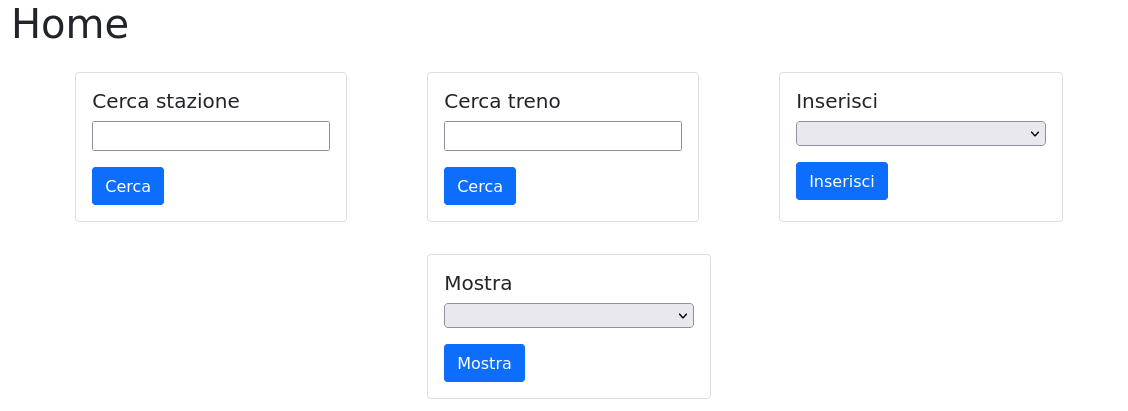
\includegraphics[width=\linewidth]{res/screenshots/home.png}
	\par Dalla homepage si puo accedere alle 2 funzioni principali di gestione del database: inserimento e ricerca,
	selezionando tramite un menu drop-down la tabella o view interessata.
	\par Si puo inoltre accedere a informazioni su treni e stazioni, con una ricerca con suggerimenti.
	\subsection{Inserimento}
	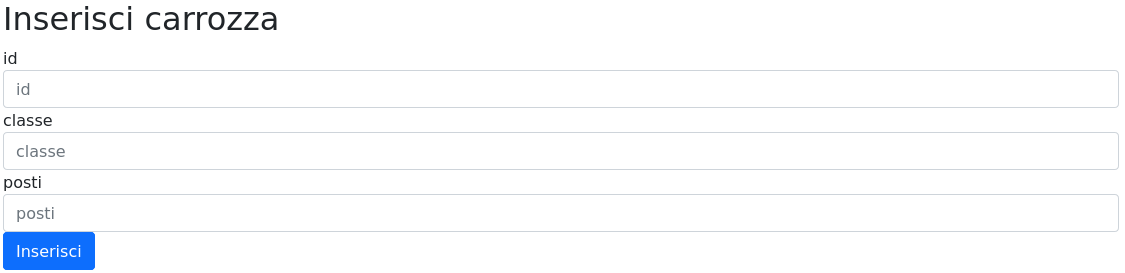
\includegraphics[width=\linewidth]{res/screenshots/inserisci.png}
	\par Nella pagina di inserimento, per ogni tabella, si puo compilare un form per inserire una riga alla tabella.
	\par Per foreign key presenti nella tabella, vengono suggeriti i valori da inserire.
	\subsection{Ricerca}
	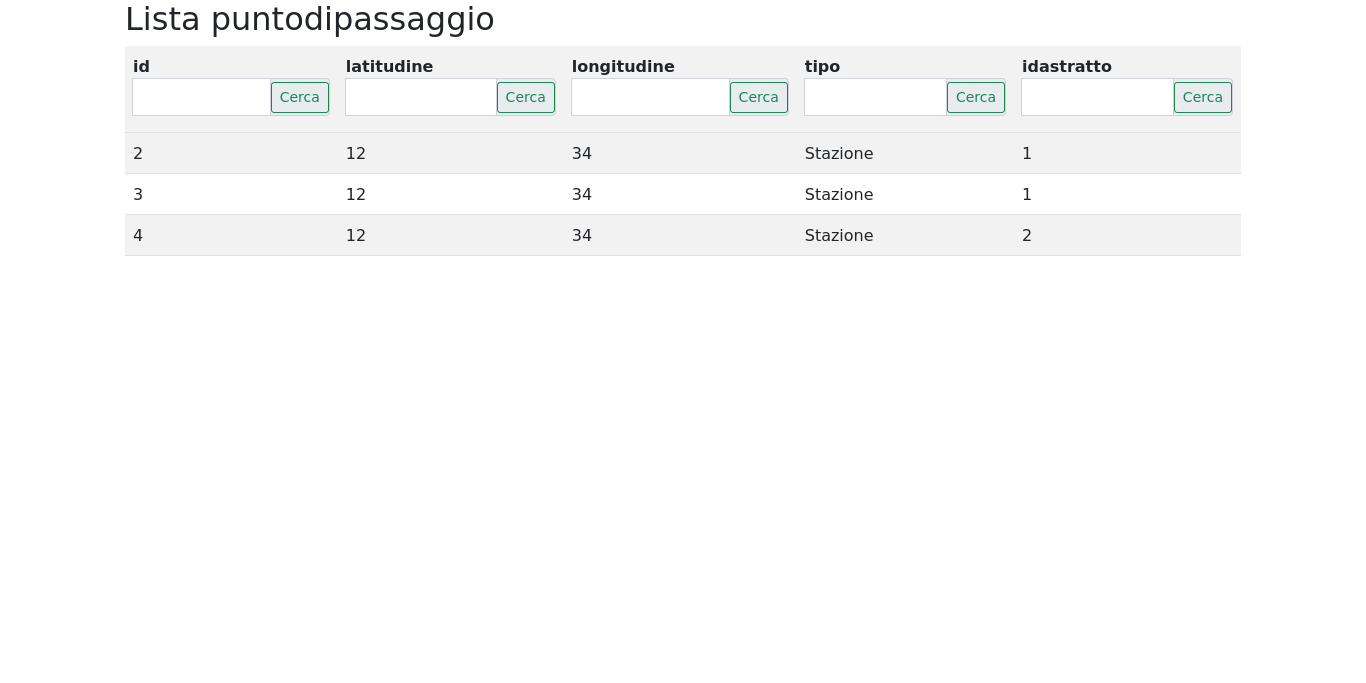
\includegraphics[width=\linewidth]{res/screenshots/lista.png}
	\par Nella pagina di ricerca viene visualizzata la tabella interessata.
	\par E' possibile eseguire una ricerca per una qualsiasi colonna della tabella.
	\subsection{Ricerca stazione}
	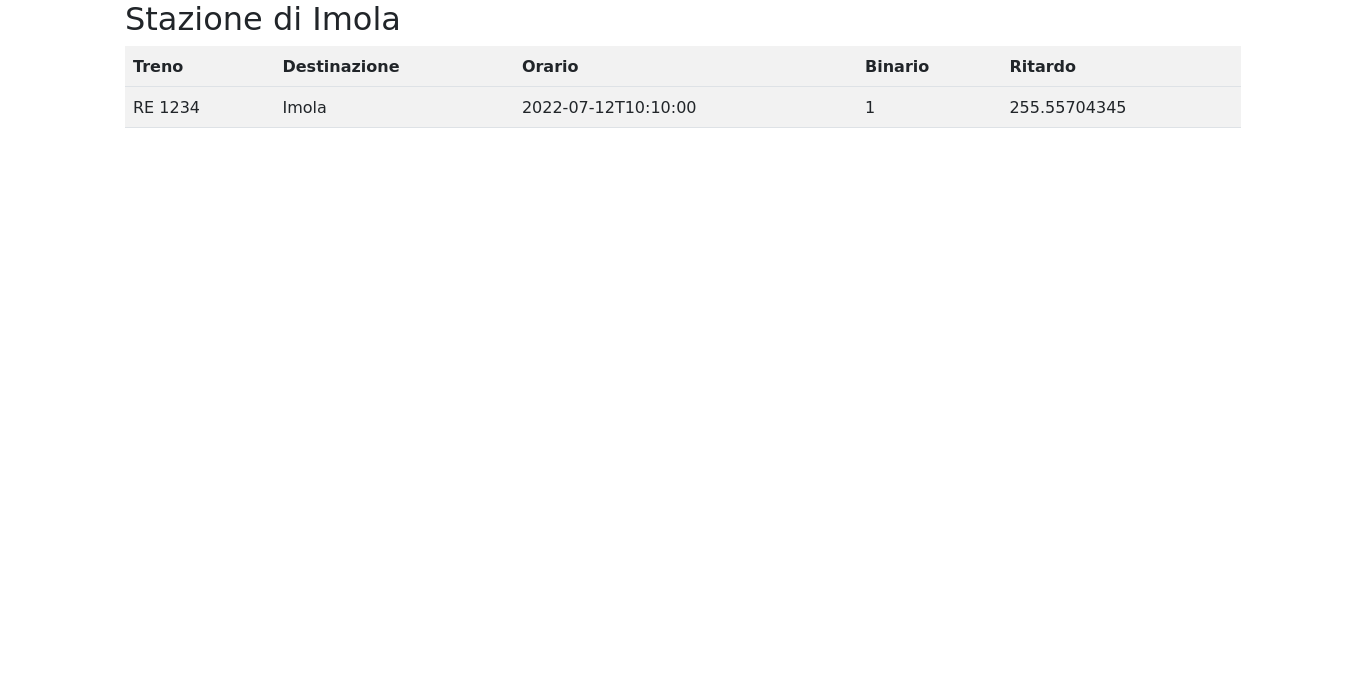
\includegraphics[width=\linewidth]{res/screenshots/stazione.png}
	\par Nella pagina relativa alla ricerca della stazione si puo vedere la lista dei treni che passano dalla stazione e alcune informazioni relative ad essi.
	\par Se si clicca sul numero del treno, si va alla pagina dello stato del treno nel giorno corrente.
	\subsection{Ricerca treno}
	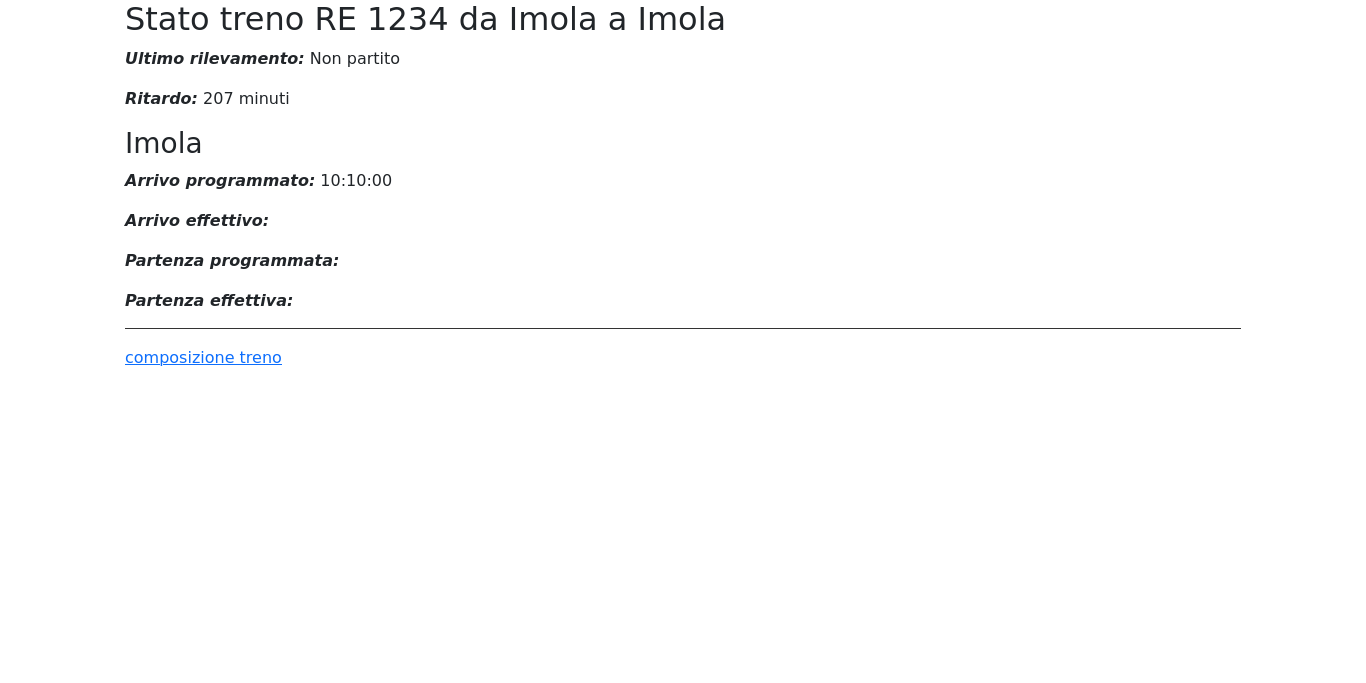
\includegraphics[width=\linewidth]{res/screenshots/stato_treno.png}
	\par Nella pagina relativa alla ricerca del treno si possono vedere informazioni logistiche relative allo stato del treno.
	\par E' anche presente un link che manda a una pagina per visualizzare la composizione del treno stesso.
    %\printbibliography[heading=bibintoc]
\end{document}
